%% =======================================================
%% Actividad 20: Proyecto de pruebas estadísticas paramétricas y no paramétricas
%%
%% Compilar desde actividades/: ./compilar.sh act20
%% Las figuras de img/ se generan con: python act20.py
%% =======================================================

%% ---- CONFIGURACIÓN ------------------------

\documentclass[11pt,letterpaper]{article}

\usepackage[indice]{tecnm}
\usepackage[T1]{fontenc}
\usepackage{amsmath}
\usepackage{xcolor}
\usepackage[most]{tcolorbox} % Carga tcolorbox con soporte para listings y saltos de página
\tcbuselibrary{listings, skins, breakable}
\setlength{\emergencystretch}{3em} % Evita líneas desbordadas por palabras en \texttt

% Paleta de colores (estilo GitHub Light / VS Code)
\definecolor{codebg}{HTML}{F8F9FA}       % Fondo del código
\definecolor{codehead}{HTML}{E9ECEF}     % Fondo de la barra de título
\definecolor{codeborder}{HTML}{CED4DA}   % Borde de la tarjeta
\definecolor{codetitle}{HTML}{212529}    % Texto del título
\definecolor{codekw}{HTML}{0550AE}       % Palabras clave (import, def, for...)
\definecolor{codefunc}{HTML}{8250DF}     % Funciones y métodos (describe, groupby...)
\definecolor{codestr}{HTML}{0A3069}      % Strings
\definecolor{codecomm}{HTML}{6E7781}     % Comentarios
\definecolor{codenum}{HTML}{8C959F}      % Números de línea
\definecolor{codeid}{HTML}{24292F}       % Texto general

% Configuración base de listings
\lstdefinestyle{pythonestilo}{
  language=Python,
  basicstyle=\ttfamily\footnotesize\color{codeid},
  keywordstyle=\color{codekw}\bfseries,
  keywordstyle=[2]\color{codefunc}, % Estilo secundario para métodos de datos
  stringstyle=\color{teal!80!black},
  commentstyle=\color{codecomm}\itshape,
  morekeywords={as, True, False, None, with, yield, lambda},
  morekeywords=[2]{f_oneway, ppf, sf, studentized_range, shapiro, rankdata, DataFrame,  boxplot, default_rng, normal, load_iris, mean, sqrt, concatenate, print, len, sum, max, DataFrame, Series, value_counts, reindex, mean, std, var, randint, normal, seed, cumsum, poisson, binom, pmf, norm, fit, kde, bincount, linspace, train_test_split, make_blobs, GaussianNB, chisquare, pdf, cdf, hist, bar, plot, axhline, axvline, fill_between, subplots, figure, concat, nunique, load_iris, diff, sort, unique},
  numbers=left,
  numberstyle=\tiny\ttfamily\color{codenum},
  stepnumber=1,
  numbersep=10pt,
  showstringspaces=false,
  morestring=[b]{"""},
  tabsize=4,
  breaklines=true,
  breakatwhitespace=true,
  columns=flexible,
  keepspaces=true,
  literate=
    {á}{{\'a}}1 {é}{{\'e}}1 {í}{{\'i}}1 {ó}{{\'o}}1 {ú}{{\'u}}1
    {Á}{{\'A}}1 {É}{{\'E}}1 {Í}{{\'I}}1 {Ó}{{\'O}}1 {Ú}{{\'U}}1
    {ñ}{{\~n}}1 {Ñ}{{\~N}}1 {¿}{{?`}}1 {¡}{{!`}}1 {°}{{$^\circ$}}1
}

% Definición del entorno personalizado \begin{codigo}{Título}{etiqueta}
% \newtcblisting[auto counter, number within=section]{codigo}[2][]{
\newtcblisting[auto counter]{codigo}[2][]{
  listing only,
  breakable,                    % Permite que el bloque se divida si pasa de página
  enhanced,
  colback=codebg,
  colframe=codeborder,
  colbacktitle=codehead,
  coltitle=codetitle,
  fonttitle=\bfseries\small\sffamily,
  boxrule=0.6pt,
  arc=4pt,                      % Bordes redondeados
  left=20pt,                    % Espacio izquierdo para los números de línea
  right=8pt,
  top=6pt,
  bottom=6pt,
  toptitle=4pt,
  bottomtitle=4pt,
  before skip=12pt,
  after skip=12pt,
  listing options={style=pythonestilo},
  title={Código \thetcbcounter: #2},
  #1
}

% Paleta para salida de consola (estilo terminal limpia)
\definecolor{termbg}{HTML}{212529}      % Fondo oscuro tipo terminal
\definecolor{termhead}{HTML}{343A40}    % Barra superior
\definecolor{termtext}{HTML}{F8F9FA}    % Texto claro de alta legibilidad
\definecolor{termborder}{HTML}{495057}  % Borde

% Entorno \begin{consola}[label=out:iris]{Título}
\newtcblisting[auto counter]{consola}[2][]{
  listing only,
  breakable,
  colback=termbg,
  colframe=termborder,
  colbacktitle=termhead,
  coltitle=termtext,
  colupper=termtext,
  fonttitle=\bfseries\small\sffamily,
  boxrule=0.6pt,
  arc=4pt,
  left=8pt,
  right=8pt,
  top=6pt,
  bottom=6pt,
  toptitle=4pt,
  bottomtitle=4pt,
  before skip=12pt,
  after skip=12pt,
  listing options={
    basicstyle=\ttfamily\scriptsize\color{termtext}, % \scriptsize evita que las tablas de Pandas se partan de línea
    breaklines=true,
    columns=fixed,        % Mantiene alineadas las columnas de Pandas
    keepspaces=true,
    showstringspaces=false,
    literate=
      {á}{{\'a}}1 {é}{{\'e}}1 {í}{{\'i}}1 {ó}{{\'o}}1 {ú}{{\'u}}1
      {Á}{{\'A}}1 {É}{{\'E}}1 {Í}{{\'I}}1 {Ó}{{\'O}}1 {Ú}{{\'U}}1
      {ñ}{{\~n}}1 {Ñ}{{\~N}}1 {°}{{$^\circ$}}1
  },
  title={Salida \thetcbcounter: #2},
  #1
}

%% ---- DATOS DE LA MATERIA ------------------------

\materia{Modelos Estadísticos para el Aprendizaje \\ Automático y Ciencia de Datos}
\actividad{Tema 3.2 Pruebas de Hipótesis Paramétricas y no Paramétricas \\ Actividad 20 - Proyecto: Comparación de múltiples clasificadores}

\profesor{Dr. José Ismael Ojeda Campaña}
%\fecha{15 de octubre de 2026}    % opcional; por defecto es la fecha de hoy

\begin{document}
\portada
\indicegeneral

%% ---- CONTENIDO ---------------------------------

\section{Introducción}

Para saber si un modelo es estadísticamente mejor que otro no basta comparar su desempeño promedio: hay que decidir si la diferencia observada es mayor de lo que produciría la variabilidad natural de los datos. Cuando se comparan más de dos clasificadores, esa decisión se toma con una prueba que contrasta todos a la vez, y el tema 3.2 distingue dos familias de pruebas según la naturaleza de los datos: las paramétricas, que suponen una distribución conocida, y las no paramétricas, que se basan en rangos \parencite{tecnm2026_tema32}.

Este proyecto compara cuatro variantes del clasificador C4.5 evaluadas en 14 conjuntos de datos, con la métrica y los datos de la Tabla~6 del trabajo de \textcite{demsar2006} y siguiendo el capítulo 13 de \textcite{walpole2007}. Se aplican tres tareas: el ANOVA (prueba paramétrica, bajo el supuesto de normalidad), la prueba de Friedman (no paramétrica) y las pruebas post-hoc de Tukey (paramétrica) y Nemenyi (no paramétrica). El ANOVA y la de Friedman solo dicen si hay alguna diferencia entre los clasificadores; las post-hoc dicen cuáles difieren. Como los cuatro clasificadores se evaluaron en los mismos conjuntos de datos, el ANOVA se aplica en sus dos versiones, de un factor y con bloques, para ver el efecto de respetar ese emparejamiento.

\section{Marco conceptual}

\subsection{Condiciones de las pruebas paramétricas}

Las pruebas paramétricas requieren que las observaciones sean independientes, que provengan de poblaciones con distribución normal y que las poblaciones tengan varianzas iguales; son confiables aun con ligeras desviaciones de la normalidad, en particular con muestras grandes \parencite{tecnm2026_tema32}. El mismo documento advierte que en aprendizaje automático es poco frecuente poder asumir normalidad e independencia, por ejemplo cuando se usa validación cruzada \parencite{tecnm2026_tema32}.

\subsection{ANOVA de un factor}

El ANOVA de un factor, o diseño completamente al azar, contrasta $H_0\colon \mu_1 = \mu_2 = \dots = \mu_k$ contra $H_1$: al menos dos medias son distintas, con $k$ muestras aleatorias independientes de poblaciones normales con varianza común \parencite[sec.~13.3]{walpole2007}. La variabilidad total se descompone como $SST = SSA + SSE$, donde $SSA$ es la variabilidad entre tratamientos y $SSE$ la variabilidad dentro de ellos. Si $H_0$ es cierta, el cociente de las medias cuadráticas
\[
f = \frac{SSA/(k-1)}{SSE/\,[k(n-1)]}
\]
sigue una distribución $F$ con $k-1$ y $k(n-1)$ grados de libertad, y se rechaza $H_0$ si $f > f_\alpha$, es decir, si $p \le \alpha$ \parencite[sec.~13.3]{walpole2007}.

\subsection{ANOVA con bloques}

Cuando los tratamientos se comparan dentro de unidades emparejadas (los bloques), el diseño por bloques completamente aleatorios separa además la variabilidad debida a los bloques: $SST = SSA + SSB + SSE$. El estadístico es $f = \dfrac{SSA/(k-1)}{SSE/[(b-1)(k-1)]}$, con $k-1$ y $(b-1)(k-1)$ grados de libertad \parencite[sec.~13.9]{walpole2007}. Quitar $SSB$ del error hace la prueba más sensible cuando los bloques difieren mucho entre sí. Aquí cada conjunto de datos es un bloque.

\subsection{Prueba de Friedman}

La prueba de Friedman es la alternativa no paramétrica al ANOVA con bloques: en lugar de los valores de desempeño usa sus rangos. En cada conjunto de datos se ordenan los $k$ clasificadores (rango 1 al mejor, y rango promedio en caso de empate) y se calcula el rango promedio $R_j$ de cada clasificador sobre los $N$ conjuntos. Bajo $H_0$ (todos los clasificadores son equivalentes) los rangos promedio son iguales, y el estadístico
\[
\chi^2_F = \frac{12N}{k(k+1)}\left[\sum_j R_j^2 - \frac{k(k+1)^2}{4}\right]
\]
sigue aproximadamente una distribución $\chi^2$ con $k-1$ grados de libertad \parencite{demsar2006}. \textcite{demsar2006} recomienda además la corrección de Iman y Davenport, $F_F = \dfrac{(N-1)\chi^2_F}{N(k-1)-\chi^2_F}$, que sigue una $F$ con $k-1$ y $(k-1)(N-1)$ grados de libertad y es menos conservadora. Como usa rangos y no los valores, no requiere normalidad \parencite{tecnm2026_tema32}. Teóricamente tiene menos potencia que el ANOVA cuando los supuestos de este se cumplen, pero no necesariamente cuando no se cumplen \parencite{demsar2006}.

\subsection{Pruebas post-hoc: Tukey y Nemenyi}

Si el ANOVA o Friedman rechazan $H_0$, hay que identificar qué pares difieren. La prueba de Tukey (paramétrica) declara distintas dos medias si su diferencia supera $q_\alpha(k, gl_e)\sqrt{CME/n}$, con $q_\alpha$ de la distribución del rango studentizado \parencite[sec.~13.6]{walpole2007}. La prueba de Nemenyi es su equivalente no paramétrico: dos clasificadores difieren si sus rangos promedio se separan más que la diferencia crítica
\[
CD = q_\alpha\sqrt{\frac{k(k+1)}{6N}},
\]
con $q_\alpha$ el valor crítico del rango studentizado dividido entre $\sqrt{2}$ \parencite{demsar2006}. La prueba de Nemenyi es análoga a la de Tukey y se usa cuando se comparan todos los clasificadores entre sí \parencite{demsar2006}.

\subsection{Críticas al ANOVA en la comparación de clasificadores}

Para comparar clasificadores en varios conjuntos de datos, \textcite{demsar2006} describe el ANOVA de medidas repetidas, que divide la variabilidad en la debida a los clasificadores, a los conjuntos de datos y al error, y propone Tukey como prueba post-hoc. Sin embargo, advierte que sus supuestos probablemente se violan con algoritmos de aprendizaje: no hay garantía de que las medidas de desempeño se distribuyan normalmente (aunque lo considera un problema menor) y, más importante, el supuesto de esfericidad (semejante a la homogeneidad de varianzas) no puede darse por hecho. Concluye que el ANOVA no parece una prueba global adecuada para los estudios típicos de aprendizaje automático, y recomienda la de Friedman con sus pruebas post-hoc \parencite{demsar2006}. En este proyecto el ANOVA se aplica como se pide, bajo el supuesto de normalidad, y se verifica ese supuesto.

\section{Descripción de la actividad}

\textbf{Objetivo:} Aplicar el estadístico paramétrico y no paramétrico en la comparación de múltiples clasificadores \parencite{tecnm2026_tema32}.

El proyecto consta de tres tareas, aplicadas a la Tabla~\ref{tab:datos}:

\begin{description}
    \item[Tarea 1: ANOVA (paramétrica).] Aplicar la prueba ANOVA para comparar los resultados, bajo el supuesto de que los datos siguen una distribución normal, apoyándose en \textcite{demsar2006} y \textcite{walpole2007}.
    \item[Tarea 2: Friedman (no paramétrica).] Aplicar la prueba de Friedman a los mismos datos y discutir sus resultados a la luz de los de la Tarea 1.
    \item[Tarea 3: Post-hoc.] Aplicar las pruebas de Tukey (paramétrica) y Nemenyi (no paramétrica), que son equivalentes, para determinar cuál de los clasificadores es mejor.
\end{description}

\begin{table}[htbp]
\centering
\caption{Área bajo la curva ROC (AUC) de cuatro variantes de C4.5 en 14 conjuntos de datos \parencite{demsar2006}.}
\label{tab:datos}
\small
\renewcommand{\arraystretch}{1.15}
\begin{tabular}{lcccc}
\hline
\textbf{Conjunto de datos} & \textbf{C4.5} & \textbf{C4.5+m} & \textbf{C4.5+cf} & \textbf{C4.5+m+cf} \\
\hline
adult (sample) & 0.763 & 0.768 & 0.771 & 0.798 \\
breast cancer & 0.599 & 0.591 & 0.590 & 0.569 \\
breast cancer wisconsin & 0.954 & 0.971 & 0.968 & 0.967 \\
cmc & 0.628 & 0.661 & 0.654 & 0.657 \\
ionosphere & 0.882 & 0.888 & 0.886 & 0.898 \\
iris & 0.936 & 0.931 & 0.916 & 0.931 \\
liver disorders & 0.661 & 0.668 & 0.609 & 0.685 \\
lung cancer & 0.583 & 0.583 & 0.563 & 0.625 \\
lymphography & 0.775 & 0.838 & 0.866 & 0.875 \\
mushroom & 1.000 & 1.000 & 1.000 & 1.000 \\
primary tumor & 0.940 & 0.962 & 0.965 & 0.962 \\
rheum & 0.619 & 0.666 & 0.614 & 0.669 \\
voting & 0.972 & 0.981 & 0.975 & 0.975 \\
wine & 0.957 & 0.978 & 0.946 & 0.970 \\
\hline
\end{tabular}
\end{table}

Según \textcite{demsar2006}, los valores de la Tabla~\ref{tab:datos} son el AUC promediado sobre una validación cruzada de cinco pliegues. C4.5 es la versión con $m = 0$ y $cf = 0.25$; en C4.5+m se ajusta $m$, en C4.5+cf se ajusta $cf$ y en C4.5+m+cf se ajustan ambos, con una validación cruzada interna de cinco pliegues \parencite{demsar2006}.

\section{Desarrollo}

Las tareas se resolvieron en el script \texttt{act20.py}, que usa \texttt{numpy}, \texttt{pandas}, \texttt{scipy} y \texttt{matplotlib}. Las sumas de cuadrados se calcularon con las fórmulas de \textcite{walpole2007} y el resultado del ANOVA de un factor se verificó con \texttt{scipy.stats.f\_oneway}. Las figuras se guardan como imágenes PNG en la carpeta \texttt{img/}. El Código~\ref{cod:comun} contiene las importaciones, el nivel de significancia $\alpha = 0.05$ y la función auxiliar \texttt{guardar()}, que además muestra las figuras en pantalla cuando el código se ejecuta en un cuaderno. El cuaderno interactivo puede consultarse en Google Colab:

\begin{center}
    \url{https://colab.research.google.com/drive/11f7rY9TMMUlbsRClcDu8o3UzlFyyXBsH?usp=sharing}
\end{center}

\begin{codigo}[label=cod:comun]{Importaciones y función auxiliar}
import os

import matplotlib

# En Colab o Jupyter no existe __file__; ahí las figuras también se muestran en pantalla
EN_NOTEBOOK = '__file__' not in globals()
if not EN_NOTEBOOK:
    matplotlib.use('Agg')  # Como script, genera las figuras como archivos PNG sin abrir ventanas

import matplotlib.pyplot as plt
import numpy as np
import pandas as pd
from scipy import stats

pd.set_option('display.width', 120)
ALFA = 0.05

# Carpeta donde se guardan las figuras que se incluyen en el reporte
BASE = os.getcwd() if EN_NOTEBOOK else os.path.dirname(os.path.abspath(__file__))
CARPETA_IMG = os.path.join(BASE, 'img')
os.makedirs(CARPETA_IMG, exist_ok=True)


def guardar(nombre):
    """Guarda la figura actual en la carpeta img/ y la muestra si se ejecuta en un notebook."""
    plt.tight_layout()
    plt.savefig(os.path.join(CARPETA_IMG, nombre), dpi=150)
    if EN_NOTEBOOK:
        plt.show()
    plt.close()
\end{codigo}

\subsection{Datos}

La Tabla~\ref{tab:datos} se transcribió al \texttt{DataFrame} del Código~\ref{cod:t1}: cada fila es un conjunto de datos ($b = 14$) y cada columna un clasificador ($k = 4$).

\begin{codigo}[label=cod:t1]{Datos}
# AUC de cuatro variantes del clasificador C4.5 en 14 conjuntos de datos
# (tabla del enunciado, Tabla 6 de Demsar, 2006). Cada fila es un conjunto de datos.
clasificadores = ['C4.5', 'C4.5+m', 'C4.5+cf', 'C4.5+m+cf']
datos = pd.DataFrame(
    [[0.763, 0.768, 0.771, 0.798],   # adult (sample)
     [0.599, 0.591, 0.590, 0.569],   # breast cancer
     [0.954, 0.971, 0.968, 0.967],   # breast cancer wisconsin
     [0.628, 0.661, 0.654, 0.657],   # cmc
     [0.882, 0.888, 0.886, 0.898],   # ionosphere
     [0.936, 0.931, 0.916, 0.931],   # iris
     [0.661, 0.668, 0.609, 0.685],   # liver disorders
     [0.583, 0.583, 0.563, 0.625],   # lung cancer
     [0.775, 0.838, 0.866, 0.875],   # lymphography
     [1.000, 1.000, 1.000, 1.000],   # mushroom
     [0.940, 0.962, 0.965, 0.962],   # primary tumor
     [0.619, 0.666, 0.614, 0.669],   # rheum
     [0.972, 0.981, 0.975, 0.975],   # voting
     [0.957, 0.978, 0.946, 0.970]],  # wine
    index=['adult', 'breast cancer', 'breast cancer wisconsin', 'cmc', 'ionosphere', 'iris',
           'liver disorders', 'lung cancer', 'lymphography', 'mushroom', 'primary tumor',
           'rheum', 'voting', 'wine'],
    columns=clasificadores)
X = datos.to_numpy()
b, k = X.shape  # b conjuntos de datos (bloques), k clasificadores (tratamientos)

print("=== Datos ===")
print(f"Conjuntos de datos (b) = {b}; clasificadores (k) = {k}")
print(pd.DataFrame({'media': datos.mean(), 'desv. est.': datos.std(ddof=1)}).round(4).to_string())
\end{codigo}

\begin{consola}[label=out:t1]{Ejecución de \texttt{act20.py}: datos}
=== Datos ===
Conjuntos de datos (b) = 14; clasificadores (k) = 4
            media  desv. est.
C4.5       0.8049      0.1602
C4.5+m     0.8204      0.1586
C4.5+cf    0.8088      0.1676
C4.5+m+cf  0.8272      0.1545
\end{consola}

Los AUC medios son 0.8049 (C4.5), 0.8204 (C4.5+m), 0.8088 (C4.5+cf) y 0.8272 (C4.5+m+cf): la mejor variante supera a la base por 0.022. En cambio, las desviaciones estándar son de unos 0.16 en todos los clasificadores, porque el AUC va de 0.56 a 1.00 según el conjunto de datos. Esa dispersión entre conjuntos es mucho mayor que las diferencias entre clasificadores, y condiciona el resultado del ANOVA.

\subsection{Tarea 1: ANOVA}

\subsubsection{ANOVA de un factor}

Las hipótesis son $H_0\colon \mu_{C4.5} = \mu_{C4.5+m} = \mu_{C4.5+cf} = \mu_{C4.5+m+cf}$ y $H_1$: al menos dos medias son distintas, con $\alpha = 0.05$. El Código~\ref{cod:t2} trata las cuatro columnas como muestras independientes de tamaño 14.

\begin{codigo}[label=cod:t2]{Tarea 1a: ANOVA de un factor}
# H0: mu_1 = mu_2 = mu_3 = mu_4     H1: al menos dos medias son distintas
# Trata las 4 columnas como muestras independientes (Walpole et al., sección 13.3).
print(f"\n=== Tarea 1a: ANOVA de un factor (alfa = {ALFA}) ===")
gran_media = X.mean()
sst = ((X - gran_media) ** 2).sum()                      # variabilidad total
ssa = b * ((X.mean(axis=0) - gran_media) ** 2).sum()     # entre tratamientos
sse1 = sst - ssa                                         # dentro de tratamientos (error)
gl_a, gl_e1 = k - 1, k * (b - 1)
f1 = (ssa / gl_a) / (sse1 / gl_e1)
p1 = stats.f.sf(f1, gl_a, gl_e1)
f_critico1 = stats.f.ppf(1 - ALFA, gl_a, gl_e1)
tabla1 = pd.DataFrame({'SC': [ssa, sse1, sst], 'gl': [gl_a, gl_e1, b * k - 1],
                       'CM': [ssa / gl_a, sse1 / gl_e1, np.nan], 'F': [f1, np.nan, np.nan],
                       'p': [p1, np.nan, np.nan]},
                      index=['Entre clasificadores', 'Error', 'Total'])
print(tabla1.round(6).to_string())
print(f"F crítico F(0.05; {gl_a}, {gl_e1}) = {f_critico1:.4f}")
print(f"Verificación con scipy: F = {stats.f_oneway(*X.T).statistic:.4f}, p = {stats.f_oneway(*X.T).pvalue:.4f}")
print(f"Decisión: {'se rechaza H0' if p1 <= ALFA else 'no se rechaza H0'}")
\end{codigo}

\begin{consola}[label=out:t2]{Ejecución de \texttt{act20.py}: Tarea 1a}
=== Tarea 1a: ANOVA de un factor (alfa = 0.05) ===
                            SC  gl        CM         F         p
Entre clasificadores  0.004455   3  0.001485  0.057804  0.981555
Error                 1.336035  52  0.025693       NaN       NaN
Total                 1.340491  55       NaN       NaN       NaN
F crítico F(0.05; 3, 52) = 2.7826
Verificación con scipy: F = 0.0578, p = 0.9816
Decisión: no se rechaza H0
\end{consola}

El estadístico es $f = 0.0578$ con 3 y 52 grados de libertad, y $p = 0.9816$. Como $0.0578 < f_{0.05}(3, 52) = 2.783$ (equivalentemente, $p > \alpha$), no se rechaza $H_0$: con este análisis no hay evidencia de diferencia entre los clasificadores. La causa es que el error ($SSE = 1.336$) contiene casi toda la variabilidad entre conjuntos de datos, así que las diferencias entre clasificadores ($SSA = 0.0045$) quedan ocultas. Pero este análisis supone muestras independientes, y aquí no lo son: los cuatro valores de cada fila corresponden al mismo conjunto de datos.

\subsubsection{ANOVA con bloques}

Como los cuatro clasificadores se evaluaron en los mismos 14 conjuntos de datos, cada conjunto es un bloque y el diseño apropiado es el de bloques completamente aleatorios, que descuenta la variabilidad entre conjuntos. El Código~\ref{cod:t3} lo calcula, verifica la normalidad de los residuos con Shapiro-Wilk y genera la Figura~\ref{fig:comp}.

\begin{codigo}[label=cod:t3]{Tarea 1b: ANOVA con bloques}
# Los 4 clasificadores se evaluaron en los mismos 14 conjuntos de datos, así que las
# observaciones están emparejadas: cada conjunto de datos es un bloque
# (Walpole et al., sección 13.9, diseño por bloques completamente aleatorios).
print(f"\n=== Tarea 1b: ANOVA por bloques (alfa = {ALFA}) ===")
ssb = k * ((X.mean(axis=1) - gran_media) ** 2).sum()     # entre conjuntos de datos
sse2 = sst - ssa - ssb                                   # error tras quitar los bloques
gl_b, gl_e2 = b - 1, (k - 1) * (b - 1)
cme2 = sse2 / gl_e2
f2 = (ssa / gl_a) / cme2
p2 = stats.f.sf(f2, gl_a, gl_e2)
f_critico2 = stats.f.ppf(1 - ALFA, gl_a, gl_e2)
tabla2 = pd.DataFrame({'SC': [ssa, ssb, sse2, sst], 'gl': [gl_a, gl_b, gl_e2, b * k - 1],
                       'CM': [ssa / gl_a, ssb / gl_b, cme2, np.nan], 'F': [f2, np.nan, np.nan, np.nan],
                       'p': [p2, np.nan, np.nan, np.nan]},
                      index=['Entre clasificadores', 'Entre conjuntos de datos', 'Error', 'Total'])
print(tabla2.round(6).to_string())
print(f"F crítico F(0.05; {gl_a}, {gl_e2}) = {f_critico2:.4f}")
print(f"Proporción de la variabilidad total debida a los conjuntos de datos: {ssb / sst:.3f}")
print(f"Decisión: {'se rechaza H0' if p2 <= ALFA else 'no se rechaza H0'}")

residuos = X - X.mean(axis=0) - X.mean(axis=1, keepdims=True) + gran_media
w, p_sw = stats.shapiro(residuos.ravel())
print(f"Shapiro-Wilk de los residuos del modelo con bloques: W = {w:.4f}, p = {p_sw:.4f}")

# Figura: los valores brutos y los valores sin el efecto del conjunto de datos
centrados = X - X.mean(axis=1, keepdims=True)
fig, ejes = plt.subplots(1, 2, figsize=(11, 4.2))
ejes[0].boxplot(X, tick_labels=clasificadores)
ejes[0].set_title('AUC observada (se solapa casi todo)')
ejes[0].set_ylabel('AUC')
ejes[1].boxplot(centrados, tick_labels=clasificadores)
ejes[1].axhline(0, color='tab:red', linestyle='--', linewidth=1)
ejes[1].set_title('AUC menos la media de su conjunto de datos')
ejes[1].set_ylabel('Diferencia respecto a la media del conjunto')
guardar('comparacion_clasificadores.png')
\end{codigo}

\begin{consola}[label=out:t3]{Ejecución de \texttt{act20.py}: Tarea 1b}
=== Tarea 1b: ANOVA por bloques (alfa = 0.05) ===
                                SC  gl        CM        F         p
Entre clasificadores      0.004455   3  0.001485  4.44718  0.008818
Entre conjuntos de datos  1.323011  13  0.101770      NaN       NaN
Error                     0.013024  39  0.000334      NaN       NaN
Total                     1.340491  55       NaN      NaN       NaN
F crítico F(0.05; 3, 39) = 2.8451
Proporción de la variabilidad total debida a los conjuntos de datos: 0.987
Decisión: se rechaza H0
Shapiro-Wilk de los residuos del modelo con bloques: W = 0.9542, p = 0.0329
\end{consola}

\begin{figure}[htbp]
\centering
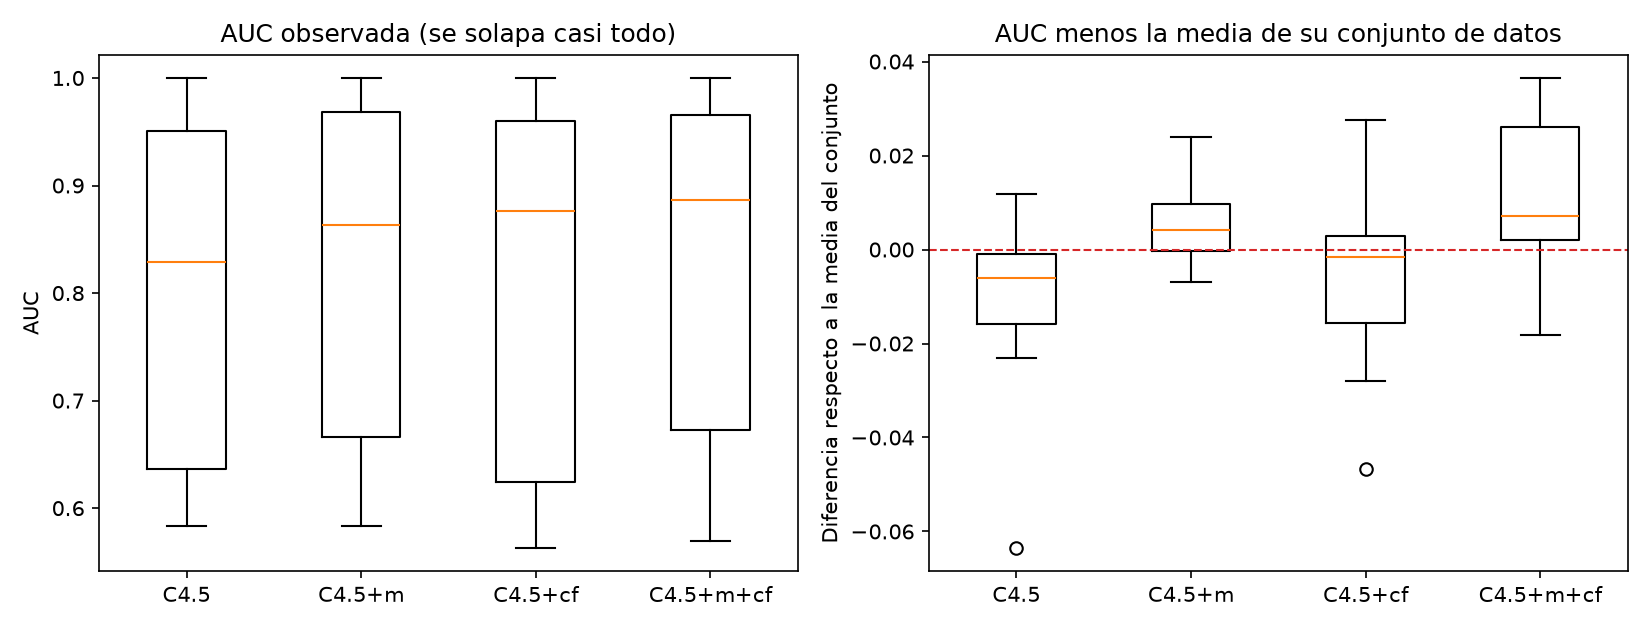
\includegraphics[width=\textwidth]{img/comparacion_clasificadores.png}
\caption{Izquierda: AUC de cada clasificador, con cajas que se solapan casi por completo. Derecha: el mismo AUC menos la media de su conjunto de datos, donde aparece la diferencia entre clasificadores.}
\label{fig:comp}
\end{figure}

Los conjuntos de datos explican el 98.7\,\% de la variabilidad total ($SSB = 1.323$ de $SST = 1.340$). Al quitarla, el error baja de 1.336 a $SSE = 0.0130$ y el estadístico pasa a $f = 4.447$ con 3 y 39 grados de libertad, con $p = 0.0088$. Como $4.447 > f_{0.05}(3, 39) = 2.845$, se rechaza $H_0$: hay evidencia de que al menos un clasificador tiene un AUC medio distinto. La suma de cuadrados entre clasificadores es la misma en los dos análisis; lo que cambia es el denominador, de $CME = 0.0257$ a $0.000334$. En la Figura~\ref{fig:comp} se ve el efecto del bloqueo: a la izquierda las cajas se solapan por completo, y a la derecha, tras descontar el conjunto de datos, C4.5+m y C4.5+m+cf quedan por encima de C4.5 y C4.5+cf.

La conclusión de la Tarea 1 es la del diseño por bloques, porque respeta el emparejamiento. Sin embargo, el supuesto de normalidad es discutible: Shapiro-Wilk sobre los residuos da $p = 0.033$, menor que 0.05.

\subsection{Tarea 2: Prueba de Friedman}

La prueba de Friedman contrasta $H_0$: los cuatro clasificadores son equivalentes, contra $H_1$: al menos uno difiere, con $\alpha = 0.05$. Usa los rangos de la tabla original (1 es el mejor AUC, con rango promedio en los empates) \parencite{demsar2006}. Son los de la publicación y no los recalculados con los valores redondeados de la tabla: en \textit{voting}, por ejemplo, C4.5+cf y C4.5+m+cf tienen ambos 0.975 pero rangos 2 y 3, lo que sugiere que se calcularon con valores sin redondear. El Código~\ref{cod:t4} transcribe los rangos y calcula $\chi^2_F$, la corrección de Iman y Davenport y una verificación con \texttt{scipy}.

\begin{codigo}[label=cod:t4]{Tarea 2: prueba de Friedman}
# H0: los k clasificadores son equivalentes (rangos promedio iguales)
# H1: al menos uno difiere. Los rangos son los de la tabla (1 = mejor AUC; empates con
# rango promedio), tal como aparecen en la Tabla 6 de Demsar (2006).
print(f"\n=== Tarea 2: prueba de Friedman (alfa = {ALFA}) ===")
rangos = pd.DataFrame(
    [[4, 3, 2, 1], [1, 2, 3, 4], [4, 1, 2, 3], [4, 1, 3, 2], [4, 2, 3, 1], [1, 2.5, 4, 2.5],
     [3, 2, 4, 1], [2.5, 2.5, 4, 1], [4, 3, 2, 1], [2.5, 2.5, 2.5, 2.5], [4, 2.5, 1, 2.5],
     [3, 2, 4, 1], [4, 1, 2, 3], [3, 1, 4, 2]],
    index=datos.index, columns=clasificadores)
R = rangos.mean()  # rango promedio de cada clasificador
print("Rangos promedio:", R.round(3).to_dict())
chi2_f = 12 * b / (k * (k + 1)) * ((R ** 2).sum() - k * (k + 1) ** 2 / 4)
p_chi = stats.chi2.sf(chi2_f, k - 1)
print(f"Friedman: chi2_F = {chi2_f:.4f}, gl = {k - 1}, p = {p_chi:.4f}")
# Corrección de Iman y Davenport (la que recomienda Demsar), menos conservadora
f_f = (b - 1) * chi2_f / (b * (k - 1) - chi2_f)
gl1, gl2 = k - 1, (k - 1) * (b - 1)
p_ff = stats.f.sf(f_f, gl1, gl2)
print(f"Iman-Davenport: F_F = {f_f:.4f}, gl = ({gl1}, {gl2}), p = {p_ff:.4f}, "
      f"F crítico = {stats.f.ppf(1 - ALFA, gl1, gl2):.4f}")
fr = stats.friedmanchisquare(*rangos.to_numpy().T)  # verificación (con corrección por empates)
print(f"Verificación con scipy (corrige empates): chi2 = {fr.statistic:.4f}, p = {fr.pvalue:.4f}")
print(f"Decisión: {'se rechaza H0' if p_ff <= ALFA else 'no se rechaza H0'}")
\end{codigo}

\begin{consola}[label=out:t4]{Ejecución de \texttt{act20.py}: Tarea 2}
=== Tarea 2: prueba de Friedman (alfa = 0.05) ===
Rangos promedio: {'C4.5': 3.143, 'C4.5+m': 2.0, 'C4.5+cf': 2.893, 'C4.5+m+cf': 1.964}
Friedman: chi2_F = 9.2786, gl = 3, p = 0.0258
Iman-Davenport: F_F = 3.6863, gl = (3, 39), p = 0.0198, F crítico = 2.8451
Verificación con scipy (corrige empates): chi2 = 10.2283, p = 0.0167
Decisión: se rechaza H0
\end{consola}

Los rangos promedio son 3.143 (C4.5), 2.000 (C4.5+m), 2.893 (C4.5+cf) y 1.964 (C4.5+m+cf), los mismos de la tabla del enunciado. Los valores $\chi^2_F = 9.28$ y $F_F = 3.69$ coinciden con los que reporta \textcite{demsar2006} para estos datos. El estadístico es $\chi^2_F = 9.279$ con 3 grados de libertad ($p = 0.0258$), y con la corrección de Iman y Davenport $F_F = 3.686$ con 3 y 39 grados de libertad, mayor que el valor crítico 2.845 ($p = 0.0198$). Se rechaza $H_0$ con ambos estadísticos. \texttt{scipy} da $\chi^2 = 10.23$ ($p = 0.0167$) porque corrige los empates; la conclusión no cambia.

\textbf{Comparación con la Tarea 1.} Friedman concuerda con el ANOVA por bloques (ambos rechazan $H_0$, con $p = 0.020$ y $p = 0.0088$) y no con el ANOVA de un factor ($p = 0.98$), porque Friedman también compara los clasificadores dentro de cada conjunto de datos y los rangos eliminan la diferencia de escala entre conjuntos. \textcite{demsar2006} reporta que Friedman y el ANOVA coinciden en la mayoría de los casos en un estudio de 56 problemas. El ANOVA con bloques tiene un valor $p$ menor, lo normal cuando los supuestos paramétricos se cumplen y la prueba usa la magnitud de las diferencias, no solo su orden. Que ambas pruebas coincidan, aunque la normalidad sea dudosa, da confianza en que la diferencia es real y no un efecto del supuesto paramétrico.

\subsection{Tarea 3: Pruebas post-hoc de Tukey y Nemenyi}

Como ambas pruebas rechazaron $H_0$, el Código~\ref{cod:t5} compara los clasificadores por pares. Tukey usa el error cuadrático medio del modelo con bloques (39 grados de libertad) y las diferencias de AUC. Nemenyi usa los rangos promedio y la diferencia crítica $CD$. También se grafica la diferencia crítica (Figura~\ref{fig:nem}).

\begin{codigo}[label=cod:t5]{Tarea 3: pruebas post-hoc de Tukey y Nemenyi}
print("\n=== Tarea 3: pruebas post-hoc ===")
# Tukey: diferencia mínima significativa con el error cuadrático medio del modelo con bloques
q = stats.studentized_range.ppf(1 - ALFA, k, gl_e2)
hsd = q * np.sqrt(cme2 / b)
print(f"Tukey: q(0.05; {k}, {gl_e2}) = {q:.4f}; diferencia mínima significativa = {hsd:.4f}")
# Nemenyi: diferencia crítica en rangos promedio, CD = q_alfa * sqrt(k(k+1) / (6 b)),
# con q_alfa = (rango studentizado con gl infinitos) / raiz(2)
q_nem = stats.studentized_range.ppf(1 - ALFA, k, np.inf) / np.sqrt(2)
cd = q_nem * np.sqrt(k * (k + 1) / (6 * b))
print(f"Nemenyi: q_alfa = {q_nem:.4f}; diferencia crítica CD = {cd:.4f}")
medias = datos.mean()
ee_rangos = np.sqrt(k * (k + 1) / (6 * b))
filas = []
for i in range(k):
    for j in range(i + 1, k):
        d_media = medias.iloc[j] - medias.iloc[i]
        d_rango = R.iloc[i] - R.iloc[j]  # positivo si j tiene mejor (menor) rango
        p_nem = stats.studentized_range.sf(abs(d_rango) / ee_rangos * np.sqrt(2), k, np.inf)
        filas.append((f"{clasificadores[j]} vs {clasificadores[i]}", d_media, abs(d_media) > hsd,
                      d_rango, p_nem, abs(d_rango) > cd))
tabla = pd.DataFrame(filas, columns=['comparación', 'dif. AUC', 'Tukey sig.',
                                     'dif. rangos', 'p Nemenyi', 'Nemenyi sig.'])
print(tabla.round(4).to_string(index=False))

# Figura: rangos promedio con la diferencia crítica de Nemenyi (1 = mejor)
fig, eje = plt.subplots(figsize=(8, 2.6))
eje.hlines(0, 1, 4, color='black')
for pos, (nombre, r) in enumerate(R.sort_values().items()):
    arriba = pos % 2 == 0
    eje.plot(r, 0, 'o', color='tab:blue')
    eje.annotate(f"{nombre} ({r:.2f})", (r, 0), xytext=(r, 0.45 if arriba else -0.45),
                 ha='center', va='bottom' if arriba else 'top',
                 arrowprops=dict(arrowstyle='-', color='gray'))
r_min, r_max = R.min(), R.max()
if r_max - r_min < cd:  # todos dentro de la diferencia crítica: una sola barra los une
    eje.hlines(-0.12, r_min, r_max, color='tab:red', linewidth=4)
eje.hlines(1.15, 1, 1 + cd, color='black', linewidth=2)
eje.text(1 + cd / 2, 1.25, f'CD = {cd:.2f}', ha='center')
eje.set_xlim(0.8, 4.2)
eje.set_ylim(-1.1, 1.6)
eje.invert_xaxis()
eje.set_yticks([])
eje.set_xlabel('Rango promedio (1 = mejor)')
for lado in ('left', 'right', 'top'):
    eje.spines[lado].set_visible(False)
guardar('diferencia_critica_nemenyi.png')
\end{codigo}

\begin{consola}[label=out:t5]{Ejecución de \texttt{act20.py}: Tarea 3}
=== Tarea 3: pruebas post-hoc ===
Tukey: q(0.05; 4, 39) = 3.7949; diferencia mínima significativa = 0.0185
Nemenyi: q_alfa = 2.5690; diferencia crítica CD = 1.2536
         comparación  dif. AUC  Tukey sig.  dif. rangos  p Nemenyi  Nemenyi sig.
      C4.5+m vs C4.5    0.0155       False       1.1429     0.0887         False
     C4.5+cf vs C4.5    0.0039       False       0.2500     0.9562         False
   C4.5+m+cf vs C4.5    0.0223        True       1.1786     0.0742         False
   C4.5+cf vs C4.5+m   -0.0116       False      -0.8929     0.2592         False
 C4.5+m+cf vs C4.5+m    0.0068       False       0.0357     0.9999         False
C4.5+m+cf vs C4.5+cf    0.0184       False       0.9286     0.2267         False
\end{consola}

\begin{figure}[htbp]
\centering
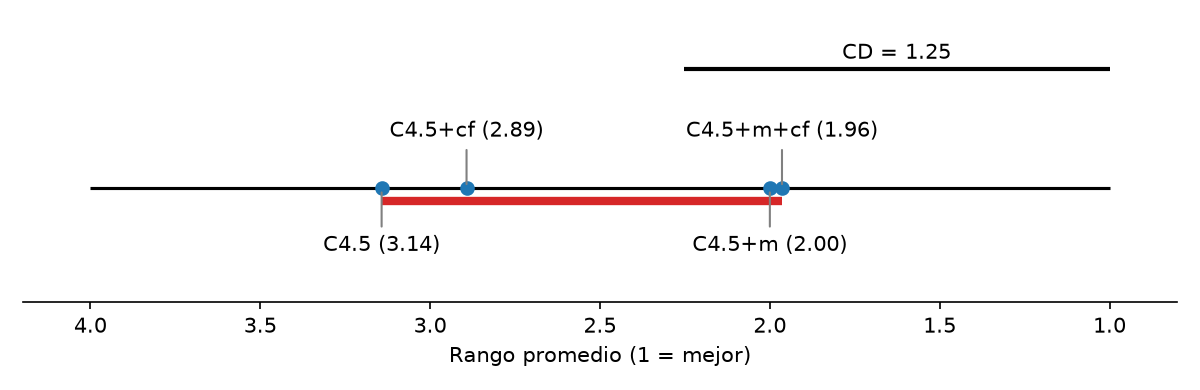
\includegraphics[width=0.85\textwidth]{img/diferencia_critica_nemenyi.png}
\caption{Rangos promedio de los clasificadores y diferencia crítica de Nemenyi ($CD = 1.25$). La barra roja une a los clasificadores que no difieren significativamente.}
\label{fig:nem}
\end{figure}

\textbf{Tukey.} La diferencia mínima significativa es $q_{0.05}(4, 39)\sqrt{CME/14} = 3.795 \times 0.00489 = 0.0185$. Solo la comparación entre C4.5+m+cf y C4.5 la supera (diferencia de AUC de 0.0223): esa variante es significativamente mejor que el clasificador base. C4.5+m+cf frente a C4.5+cf queda justo debajo del umbral (0.0184 contra 0.0185) y las demás diferencias son menores.

\textbf{Nemenyi.} La diferencia crítica es $CD = 2.569\sqrt{4 \cdot 5/(6 \cdot 14)} = 1.254$. La mayor diferencia de rangos es 1.179 (C4.5+m+cf contra C4.5, $p = 0.074$), seguida de 1.143 (C4.5+m contra C4.5, $p = 0.089$). Ninguna supera $CD$, así que Nemenyi no declara diferencias significativas entre ningún par, y en la Figura~\ref{fig:nem} los cuatro clasificadores quedan unidos por una misma barra.

\textbf{Resultado del artículo.} Con estos mismos datos, \textcite{demsar2006} obtiene también $CD = 1.25$ y concluye que Nemenyi no tiene potencia suficiente para detectar diferencias; con $p = 0.10$ ($CD = 1.12$) sí encuentra que C4.5 es peor que C4.5+m y C4.5+m+cf. Además, observa que a veces Friedman rechaza y la prueba post-hoc no detecta nada, y lo atribuye a la menor potencia de la post-hoc: en ese caso solo se puede concluir que algunos algoritmos difieren \parencite{demsar2006}. Si el interés es comparar con un control (aquí C4.5), el artículo usa Bonferroni-Dunn, con $CD = 1.16$, y C4.5+m+cf es significativamente mejor que C4.5 (diferencia de rangos 1.179), lo que coincide con el resultado de Tukey.

\textbf{Comparación.} Las dos pruebas coinciden en el orden: C4.5+m+cf y C4.5+m son los mejores (rangos 1.96 y 2.00, y AUC medios 0.827 y 0.820) y C4.5 es el peor (rango 3.14), y las dos señalan como la diferencia más grande la de C4.5+m+cf contra C4.5. Difieren en que Tukey la declara significativa y Nemenyi no. Es lo esperable: Tukey usa la magnitud de las diferencias y Nemenyi solo su orden, y por eso es más conservadora y tiene menos potencia con solo 14 conjuntos de datos. Que Nemenyi no detecte diferencias no prueba que los clasificadores sean iguales, sino que esta muestra no basta para distinguirlos por rangos.

\section{Interpretación estadística}

\textbf{¿Hay diferencia entre los clasificadores?} Sí, según las dos pruebas globales que respetan el diseño: el ANOVA con bloques ($p = 0.0088$) y Friedman ($p = 0.020$ con Iman y Davenport). El ANOVA de un factor ($p = 0.98$) no la detecta porque supone muestras independientes y mezcla la variabilidad entre conjuntos de datos con el error. Que el diseño cambie la conclusión muestra la importancia de elegir la prueba según la naturaleza de los datos \parencite{tecnm2026_tema32}.

\textbf{¿Cuál clasificador es mejor?} C4.5+m+cf es el mejor en las dos medidas: tiene el mayor AUC medio (0.8272) y el menor rango promedio (1.964), seguido de cerca por C4.5+m. La prueba de Tukey respalda que es mejor que C4.5, pero no que sea mejor que C4.5+m ni que C4.5+cf, y Nemenyi no separa a ningún par. Con estos datos, lo que se puede afirmar es que añadir los dos ajustes (m y cf) mejora al C4.5 base en unos 0.022 de AUC, y que entre las variantes la evidencia no alcanza para ordenarlas con seguridad.

\textbf{Paramétrico y no paramétrico.} Las dos familias concuerdan en lo esencial. La diferencia es de potencia: las paramétricas aprovechan la magnitud de las diferencias y detectan más, pero dependen de supuestos que aquí son dudosos (Shapiro-Wilk, $p = 0.033$; AUC acotado en $[0, 1]$; un conjunto con AUC 1.000 en todos). Además, cada valor de la tabla es un AUC promediado en una validación cruzada, cuyos conjuntos de entrenamiento se solapan, así que las observaciones no son independientes \parencite{demsar2006}. Las no paramétricas no dependen de esos supuestos pero son más conservadoras, como se vio en Nemenyi. Esto es consistente con la recomendación de \textcite{demsar2006} de usar pruebas basadas en rangos para comparar clasificadores en varios conjuntos de datos.

\section{Conclusiones}

El ANOVA de un factor ($f = 0.058$, $p = 0.98$) no encontró diferencias entre los cuatro clasificadores, pero es inadecuado porque trata como independientes datos emparejados por conjunto de datos. El ANOVA con bloques ($f = 4.447$, $p = 0.0088$) y la prueba de Friedman ($\chi^2_F = 9.28$, $p = 0.026$; $F_F = 3.69$, $p = 0.020$) sí rechazaron la igualdad, y coinciden entre sí.

En las pruebas post-hoc, Tukey mostró que C4.5+m+cf es significativamente mejor que C4.5 (0.0223 contra un umbral de 0.0185), mientras que Nemenyi, más conservadora, no encontró ningún par significativo (diferencia máxima de rangos 1.179 contra $CD = 1.254$). Ambas pruebas ordenan igual a los clasificadores, con C4.5+m+cf y C4.5+m al frente y C4.5 al final. La elección entre el enfoque paramétrico y el no paramétrico depende de si se confía en sus supuestos: aquí la normalidad es discutible, así que conviene reportar los dos resultados, como se hizo \parencite{demsar2006,tecnm2026_tema32}.

\referencias

\end{document}
